\subsubsection{GBN (Go-back-N)}

\begin{itemize}
  \item ACKの受信を待たずに、連続するパケットを最大N個まで送信可 (スライディングウィンドウ方式)
  \item 送信失敗が確認されると、そのパケットからやり直し(受信側のバッファサイズは 1)
\end{itemize}
\begin{itemize}
  \item 送信側\\
    パケットにシーケンス番号を付加  ($k$ビット)\\
    ウィンドウサイズ N(N$ < 2^k$)とタイムアウト時間を設定
  \begin{itemize}
    \item F: 送信したが、ACK未受信のパケット数
  \end{itemize}
  \begin{enumerate}
    \item 次に送るべきパケット(番号順)を F$=$N になるまで連続して送信
    \item 各パケットに対するACKを待つ
    \begin{enumerate}
      \item タイムアウト時間までにACKを受信したら、1へ
      \item タイムアウト時間までにACKを受信しなければ以降のパケットを受信失敗とみなして、1へ
    \end{enumerate}
  \end{enumerate}
  \item 受信側
  \begin{enumerate}
    \item パケットを受け取ったら、誤りがなく、正しい順序のパケットか確認
    \item 誤りがなく、正しい順序ならば、そのシーケンス番号を付加したACKを送信
    \item そうでなければ、そのパケットを破棄し、正しい順序で受け取った最後のパケットのシーケンス番号を付加したACKを送信
  \end{enumerate}
\end{itemize}

\vskip\baselineskip
\textcolor{orange}{累積ACK (Cumulative ACK)}
\begin{itemize}
  \item 付加されたシーケンス番号以前のパケットが全て正しく受信されたことを示す
  (ACKを一つにまとめる)
\end{itemize}

\begin{figure}[h]
% img: 左側はACKの失敗なし、右側は再送あり
% ウィンドウサイズ分をまとめて送信

% 一番都合の悪い場合
% 0 から 3 のパケットを受信成功したが、それに対するACKが全てロスした場合
  \centering
  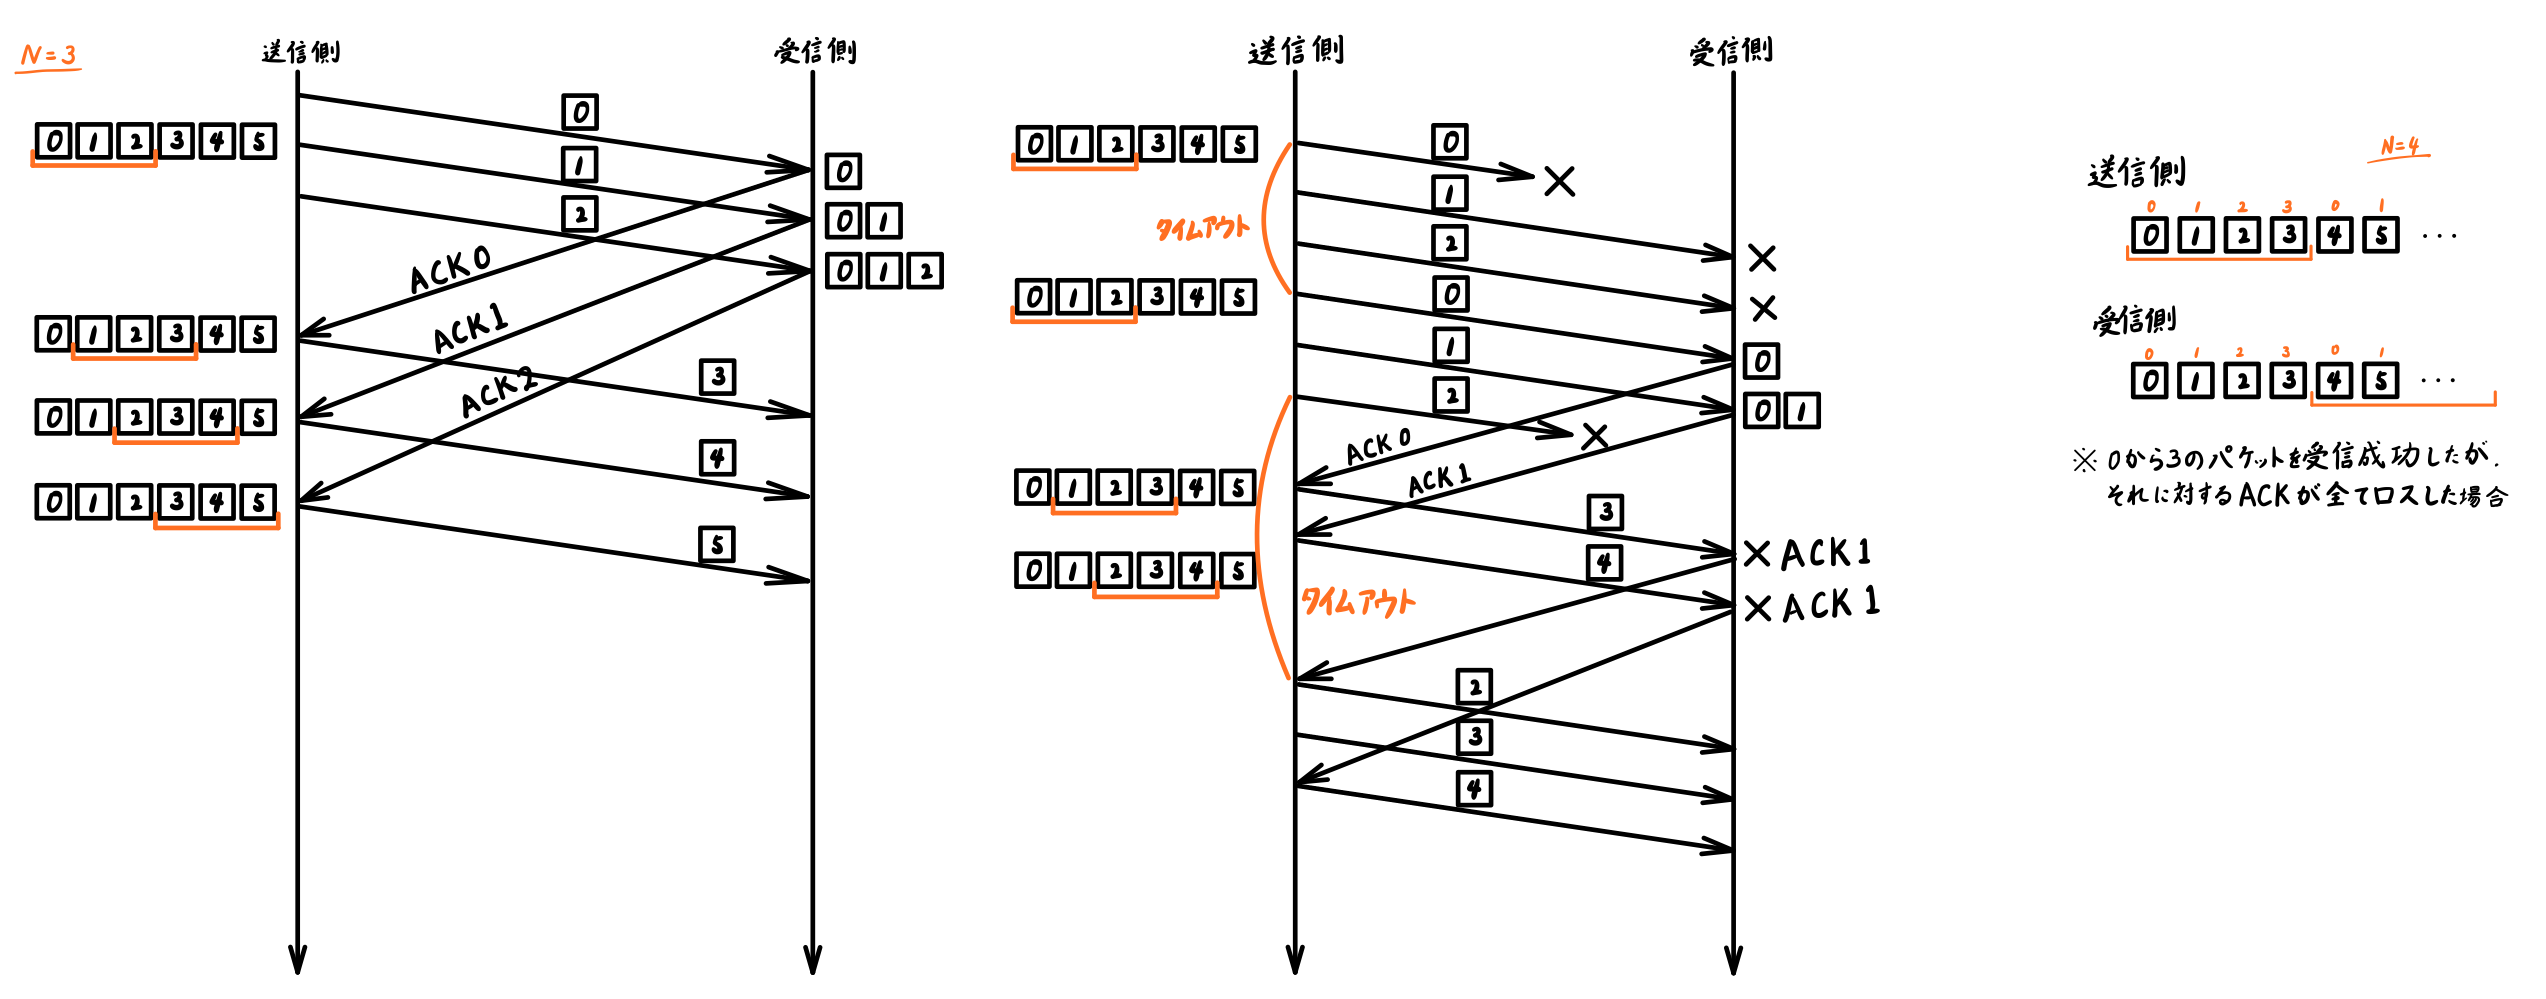
\includegraphics[width=0.9\linewidth]{image/cumulative_ack.png}
\end{figure}

\textcolor{cyan}{gbnの場合はシーケンス番号の方が(パケットサイズもしくはパケットより)1ビット大きくもつ必要がある}

\newpage
\subsubsection{SR (selective-Repeat)}

ACKの受信を待たずに連続するパケットを最大 N 個まで送信可

送信失敗が確認されると、そのパケットのみ再送  (受信バッファサイズ N)

\begin{itemize}
  \item 送信側
  \begin{itemize}
    \item パケットにシーケンス番号を付加 ($k$ ビット)
    \item ウィンドウサイズ (N $\leq 2^{k-1}$) とタイムアウト時間を設定
    \begin{itemize}
      \item n: 送信したが、ACK未受信のパケットの最小シーケンス番号
    \end{itemize}
  \end{itemize}
  \begin{enumerate}
    \item 次に送るべきパケットのうち、 $n+N-1$ 番までを連続的に送信し、2へ
    \item 各パケットに対するACKの受信を待つ
    \begin{enumerate}
      \item タイムアウト時間内にACKを受信したら、1へ
      \item タイムアウト時間内にACKを受信しなければそのパケットを再送し、2へ
    \end{enumerate}
  \end{enumerate}
  \item 受信側
  \begin{enumerate}
    \item パケットを受け取ったら、誤りがないか確認
    \item 誤りがなければ、\undercolor{そのシーケンス番号を付加したACK}
    \footnote{\textcolor{orange}{選択的(Selective) ACK}}
    を送信\\
      (順序通りに上位層へ渡すため、バッファリング)
  \end{enumerate}
\end{itemize}

\begin{figure}[h]
% img: 上記のGo-back-Nの図を編集したもの
% 左側は "SRでも同じ"
% ウィンドウ内のすべてのパケットに対応するACKが返ってきたらウィンドウを移動?
  \centering
  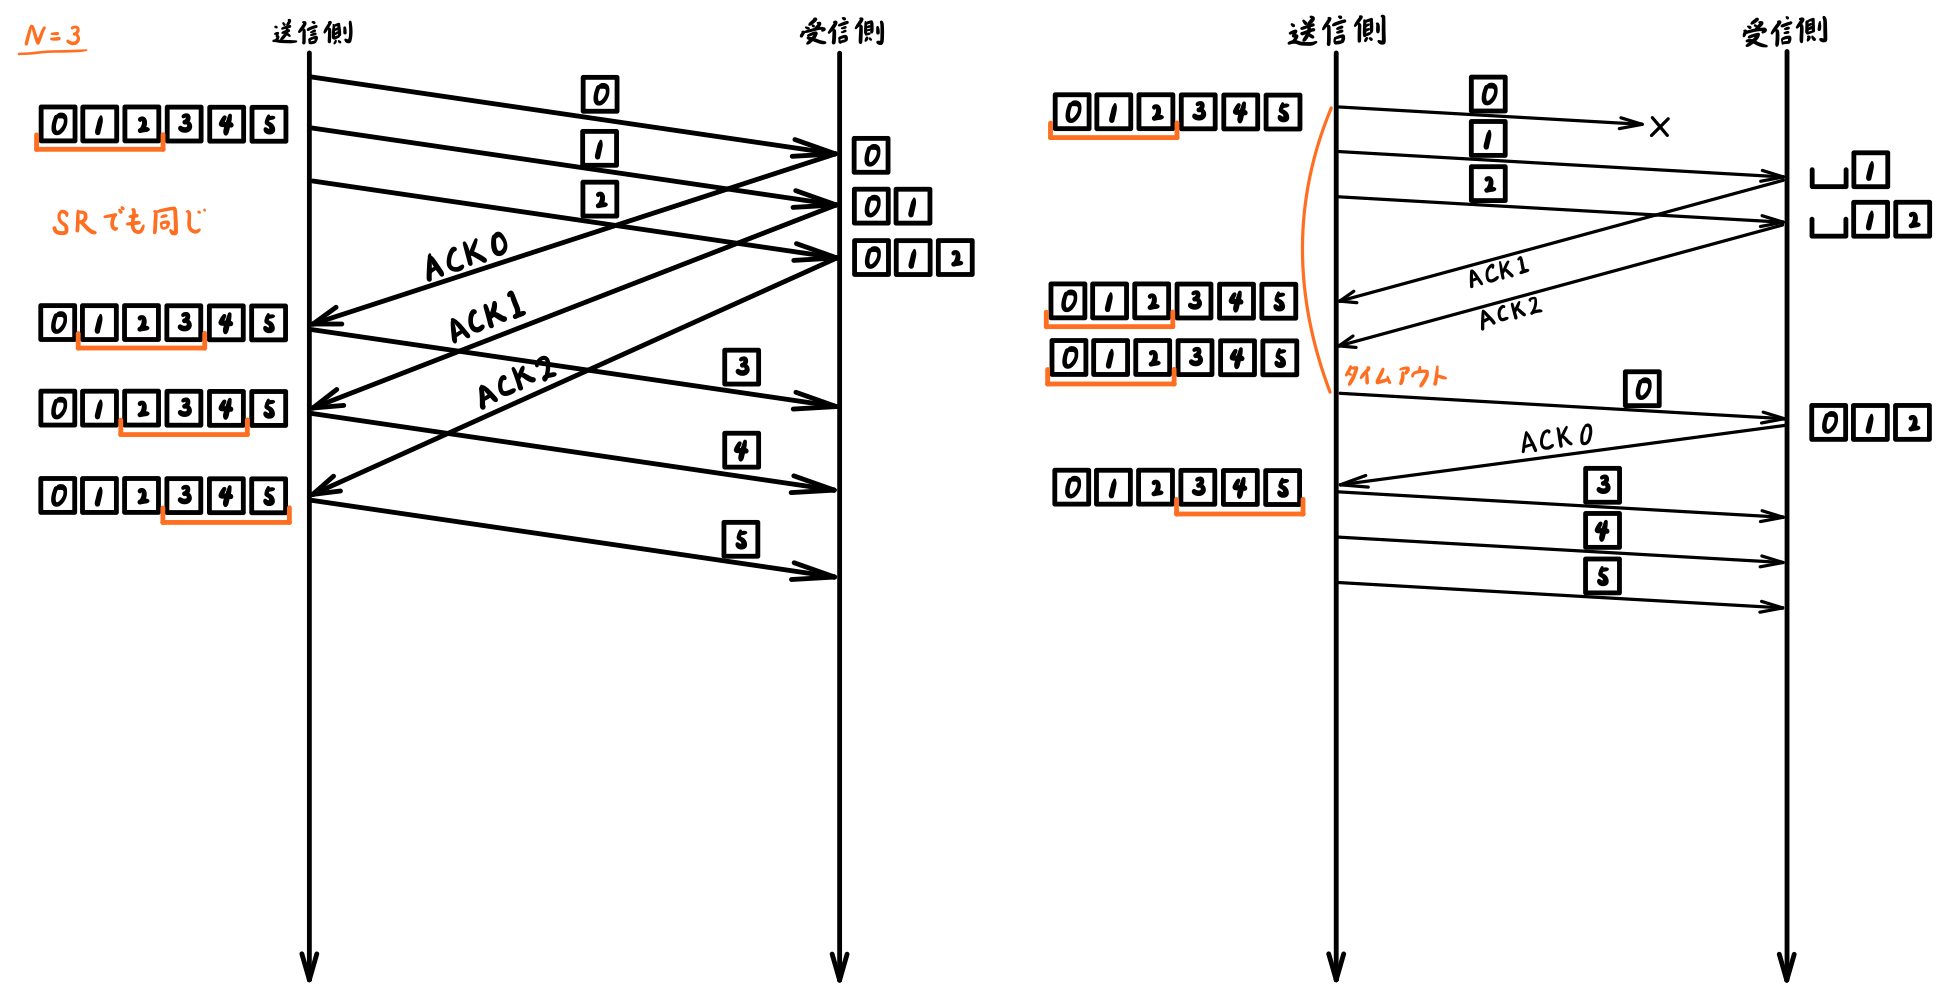
\includegraphics[width=0.8\linewidth]{image/selective_repeat.png}
\end{figure}

% 次回の頭に解説するらしい この手法が有効な場合の例?

% TCPはざっくりGo-back-Nだけど、すぐに捨てるわけじゃないみたい(前回メモ) + 輻輳制御の話に
